\documentclass{standalone}
\usepackage{tikz}
\usepackage{ctex,siunitx}
\usepackage{tkz-euclide}
\usepackage{amsmath}
\usetikzlibrary{patterns, calc}
\usetikzlibrary {decorations.pathmorphing, decorations.pathreplacing, decorations.shapes,}
\newcommand\hand[2][0]{
    \begin{scope}[#2,rotate=#1]
    \fill[pink!10!orange!10,draw=black,very thin]
    (0.113, 0.828)..controls(0.362, 0.899)and(0.627, 0.957)..
(0.754, 0.946)..controls(0.961, 0.924)and(0.983, 0.877)..
(0.961, 0.837)..controls(0.928, 0.743)and(1.042, 0.712)..
(1.000, 0.607)..controls(0.972, 0.541)and(1.011, 0.446)..
(0.930, 0.406)..controls(0.905, 0.397)and(0.911, 0.329)..
(0.844, 0.306)..controls(0.832, 0.303)and(0.838, 0.200)..
(0.779, 0.176)..controls(0.513, 0.071)and(0.348,-0.016)..(0.063, 0.177);
  \draw[very thin]
  (0.618,0.898)..controls(0.634,0.877)and(0.645,0.840)..(0.652,0.822)
  (0.550,0.870)..controls(0.569,0.863)and(0.582,0.843)..(0.584,0.830)
  (0.519,0.869)..controls(0.527,0.863)and(0.529,0.854)..(0.524,0.842)
  (0.847,0.929)..controls(0.797,0.864)and(0.833,0.717)..(0.945,0.787)
  (0.355,0.745)..controls(0.527,0.736)and(0.710,0.760)..(0.887,0.759)
  (0.704,0.501)..controls(0.789,0.544)and(0.935,0.538)..(1.000,0.607)
  (0.521,0.499)..controls(0.559,0.496)and(0.594,0.503)..(0.614,0.513)
  (0.634,0.369)..controls(0.686,0.339)and(0.726,0.346)..
  (0.802,0.377)..controls(0.845,0.390)and(0.884,0.400)..(0.930,0.406)
  (0.548,0.210)..controls(0.661,0.245)and(0.775,0.280)..(0.844,0.306)
  (0.069,0.301)..controls(0.143,0.268)and(0.232,0.253)..(0.297,0.254)
  (0.081,0.349)..controls(0.150,0.325)and(0.257,0.316)..(0.338,0.319);
  \end{scope}
  }
\begin{document}
\small
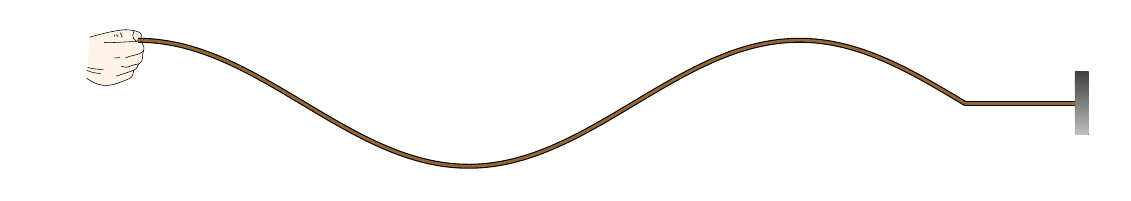
\begin{tikzpicture}[>=stealth,xscale=0.7,yscale=0.8,samples=200]
  \useasboundingbox(-2.0,1.2)rectangle(17.5,-1.1);
  \draw[fill=brown!80!black](15,0)circle(0.9pt);
  \hand{xshift=-10mm,yshift=2.2mm,xscale=1.1}
  \draw [double=brown!80!black,double distance=1pt, domain=0:15]  plot (\x,{cos(1/6*pi*\x r)});
  \draw [double=brown!80!black,double distance=1pt, domain=15:17]  plot (\x,0);
  \fill [left color=darkgray, bottom color=lightgray](17,-0.5)rectangle(17.25,0.5);
  
\end{tikzpicture}
\end{document}